\chapter{Methods and Results}

TODO:\begin{enumerate}
    \item Check for consistent notation
\end{enumerate}

\section{Description}

\subsection*{Model and Synthetic Data Simulations}

\begin{figure}[htbp]
    \centering
    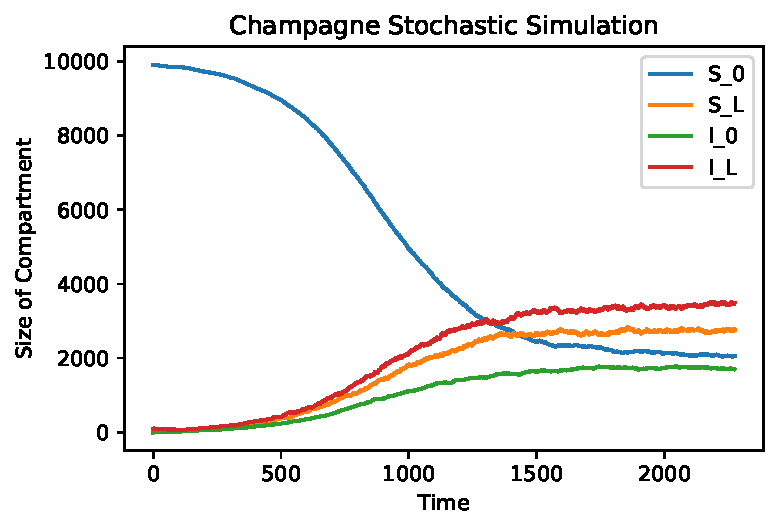
\includegraphics{../champagne_GP_images/champagne_simulation.pdf}
    \caption{A Doob-Gillespie Simulation of the model described by \cite{champagne_using_2022}.}\label{fig:champ_doob}
\end{figure}

In order to trial this method we used the model described in
\cite{champagne_using_2022}, and graphically depicted in Figure
\ref{fig:champ_diag}. Exact model simulations such as in Figure
\ref{fig:champ_doob} were computed using the
Doob-Gillespie algorithm (Algorithm \ref{alg:doob}).

Synthetic data was generated from a single run of the model, using a population
size of 1,000, an initial infected population of 10 (with both liver and blood
stage infection). The parameters used closely followed those reported in 
\cite{champagne_using_2022}: \begin{itemize}
    \item $\alpha = 0.4$
    \item $\beta = 0.4$
    \item $\gamma_L = 1 / 223$
    \item $\delta = 0$ (which we drop for the remainder of the thesis)
    \item $\lambda = 0.04$
    \item $f = 1 / 72 $
    \item $r = 1 / 60.$
\end{itemize}
The model was run for a minimum of 30 days and 15,000 events
(infections, recoveries etc.), after which time, it was assumed to have reached
equilibrium.

\subsection*{Summary Statistics and Discrepancy Function} 

Three summary statistics were extracted from the initial model run were:
\begin{enumerate}
    \item prevalence at the end of the model run - $p_\text{obs}$
    \item number of cases in the first week of the epidemic
          (first month incidence) - $m_\text{obs}$
    \item a single observation of the number of weekly cases at equilibrium
          (weekly incidence) - $w_\text{obs}.$
\end{enumerate} Similarly we extracted $p, m,$ and $w$ from each new model run.

Our discrepency function we used was the $L_1$ norm of the relative differences $$\mathcal{D}(\alpha, \beta, \gamma_L, \lambda, f, r) = \left|\frac{p - p_\text{obs}}{p_\text{obs}}\right| + \left|\frac{m - m_\text{obs}}{m_\text{obs}}\right| + \left|\frac{w - w_\text{obs}}{w_\text{obs}}\right|.$$



The acquisition function used was $$\mu(\bm\theta) - \eta_t\sqrt{\mathrm{v}(\bm\theta)}$$ with $\eta_t:= \sqrt{c + 2\ln(t^{d/2 + 2})},$ and $c$ can be chosen, $\mu(\bm\theta)$ and $\mathrm{v}(\bm\theta)$ are the posterior mean and variance
$$(\mu_\text{min} - \mu(\bm\theta))
\varPhi\left(\frac{\mu_\text{min} - \mu(\bm\theta)}{\sqrt{\mathrm{v}(\bm\theta)}}\right) + \sqrt{\mathrm{v}(\bm\theta)}
\phi\left(\frac{\mu_\text{min} - \mu(\bm\theta)}{\sqrt{\mathrm{v}(\bm\theta)}}\right)$$
$\mu_\text{min} := \min_{\bm{\theta}} \mu(\bm\theta)$
$\varPhi, \phi$ 

\subsection*{Justification}

Using relative differences limits the impact between the scale differences of the summary statistics.

\section{Running the Model and Our Choices}

Although most of the procedure we used closely follows the paper by
\cite{gutmann_bayesian_2016}, there are a few key ways in which we modified the
manuscript's method. In particular, we felt the choice of squared exponential
kernel was not a good assumption, since it implicitly assumes a high degree of
smoothness in the target discrepency function. This is unlikely to be met if
the model has any bifurcation points. To compensate for any non-smoothness in
the function, the length scale is forced to be set very small. Therefore,
although the squared exponential is the most commonly chosen kernel,
we used a Mat\'ern kernel with $\nu = 5/2$. This is not as constrained as a
squared exponential kernel, but realisations are twice mean square
differentiable.

